\documentclass[11pt]{article}

% arXiv推荐的宏包
\usepackage[utf8]{inputenc}
\usepackage[english]{babel}
\usepackage[T1]{fontenc}
\usepackage{hyperref}
\usepackage{url}

% 中文支持
\usepackage[UTF8]{ctex}

% 页面设置
\usepackage[top=1in, bottom=1in, left=1in, right=1in]{geometry}
\usepackage{parskip}

% 图形和绘图
\usepackage{graphicx}
\usepackage{grffile}  % 更好地处理文件名
\usepackage{tikz}
\usetikzlibrary{shapes,arrows.meta,positioning,fit,backgrounds,calc,shadows}

% 设置图片搜索路径
\graphicspath{{../pictures/}}

% 表格
\usepackage{booktabs}
\usepackage{tabularx}
\usepackage{array}

% 数学符号
\usepackage{amsmath}
\usepackage{amssymb}
\usepackage{amsfonts}

% 代码高亮
\usepackage{listings}
\usepackage{xcolor}
\definecolor{codegreen}{rgb}{0,0.6,0}
\definecolor{codegray}{rgb}{0.5,0.5,0.5}
\definecolor{codepurple}{rgb}{0.58,0,0.82}
\definecolor{codeblue}{rgb}{0.0,0.0,0.8}
\definecolor{backcolour}{rgb}{0.95,0.95,0.92}

\lstdefinestyle{mystyle}{
    backgroundcolor=\color{backcolour},
    commentstyle=\color{codegreen},
    keywordstyle=\color{codeblue}\bfseries,
    numberstyle=\tiny\color{codegray},
    stringstyle=\color{codepurple},
    basicstyle=\ttfamily\small,
    breakatwhitespace=false,
    breaklines=true,
    captionpos=b,
    keepspaces=true,
    numbers=left,
    numbersep=5pt,
    showspaces=false,
    showstringspaces=false,
    showtabs=false,
    tabsize=4,
    frame=single
}
\lstset{style=mystyle}

% 超链接设置
\hypersetup{
    colorlinks=true,
    linkcolor=blue,
    urlcolor=blue,
    citecolor=blue,
    pdfauthor={MoAgent Team},
    pdftitle={MoAgent: A Multi-Agent Collaborative Web Information Acquisition System},
    pdfkeywords={Multi-Agent, LLM, RAG, Web Crawling, Intelligent System}
}

% 标题信息
\title{\textbf{MoAgent: A Multi-Agent Collaborative Web Information Acquisition System}\\
\large 基于多智能体协作的网络信息获取系统}

\date{\today}

\begin{document}

\maketitle

\begin{abstract}
本报告详细介绍了MoAgent项目的架构设计与技术实现。MoAgent是一个基于多智能体协作、大语言模型(LLM)和检索增强生成(RAG)技术的智能网络信息获取系统。项目通过智能体工作流编排、自适应爬虫引擎和模式学习机制,实现了零规则启动、自动适应网站变化和持续自我优化的能力。系统采用四层架构设计,包括应用层、决策层、执行层和基础设施层,实现了高内聚、低耦合的模块化设计。核心设计包括基于LangGraph的工作流编排、多智能体协作机制、LLM语义理解和RAG向量检索技术。完整工程代码可见\url{https://github.com/Lineance/Moagent}。
\end{abstract}

\section{引言}

\subsection{项目背景}

在信息过载的时代,碎片化阅读日益普遍,导致用户注意力难以集中。尽管采用RSS订阅是一种常见的解决方案,但其支持范围有限,且往往无法完整提取全文内容。此外,现代Web开发中广泛采用React、Vue等动态渲染框架,而传统的基于BeautifulSoup的规则爬虫难以有效抓取此类动态生成的内容。与此同时,网站DOM结构频繁变更,使得手动维护爬虫规则的成本显著增加。

\subsection{项目动机}

本项目的发起源于一个具体的个人需求:尝试利用RSS技术聚合多个关键信息源,包括东南大学的重要通知、人工智能领域顶会的最新论文、小红书上的即时消息以及技术播客的内容等等。然而,在实践过程中遇到了以下突出困难:

\begin{itemize}
    \item \textbf{关键信源缺乏支持}:许多重要网站(如学校官网)并未提供原生的RSS订阅功能。
    \item \textbf{传统方法效率低下}:针对无RSS的网站,手动编写与维护内容提取规则(如CSS选择器、XPath)不仅耗时,且极其脆弱,网站结构的微小变动便会导致规则失效。
    \item \textbf{技术能力局限}:现有主流工具难以有效应对广泛使用的动态网页技术(如通过JavaScript异步加载内容列表)。
\end{itemize}

这些实际痛点引出了本项目需要解决的核心问题:能否设计并实现一个新型的网络信息获取框架,使其具备无需预设规则即可启动、能够持续自我适应网站变化,并在动态内容失效时智能回退至可靠方案的能力?

\subsection{项目目标}

为了锻炼自己的开发和设计能力,我选择系统性初步实现MoAgent,旨在系统性地学习和实践现代多智能体系统工程的基础实践拟在未来完整实现一个具备生产级质量的新闻聚合智能系统:

\begin{enumerate}
    \item 构建一个协同工作的多智能体系统(而非单一模型调用),涉及工作流编排、实时决策与多智能体分工协作
    \item 项目从定义问题(脆弱的传统爬虫)出发,通过智能体架构提供创新解法,并设计可运行的反馈学习机制
\end{enumerate}

\section{系统架构设计}

\subsection{技术依赖层次}

系统采用四层架构设计,从基础设施层到应用层逐层构建,实现高内聚、低耦合的模块化设计。图~\ref{fig:mainpage}展示了系统的整体架构,图~\ref{fig:architecture}展示了四层架构的详细设计。

\begin{figure}[htbp]
\centering
\begin{tikzpicture}[
    layer/.style={rectangle, draw, fill=blue!10, text width=12cm, minimum height=1.5cm, align=center, rounded corners},
    arrow/.style={-Stealth, thick}
]
    % 应用层
    \node[layer, fill=green!10] (app) at (0, 6) {\textbf{应用层}\\智能体工作流 (LangGraph)};

    % 决策层
    \node[layer, fill=yellow!10] (decision) at (0, 4.2) {\textbf{决策层}\\模式生成与记忆学习 (RAG + Pattern Generator)};

    % 执行层
    \node[layer, fill=orange!10] (exec) at (0, 2.4) {\textbf{执行层}\\自适应爬虫引擎 (Playwright + BeautifulSoup)};

    % 基础设施层
    \node[layer, fill=blue!10] (infra) at (0, 0.6) {\textbf{基础设施层}\\ChromaDB + SQLite + asyncio + pytest};

    % 箭头
    \draw[arrow] (app.south) -- (decision.north);
    \draw[arrow] (decision.south) -- (exec.north);
    \draw[arrow] (exec.south) -- (infra.north);
\end{tikzpicture}
\caption{Four-Layer Architecture: System design from infrastructure layer to application layer with clear separation of concerns.}
\label{fig:architecture}
\end{figure}

\begin{figure}[htbp]
\centering
\includegraphics[width=0.9\textwidth]{mainpage.png}
\caption{MoAgent System Homepage: User interface showing the four-layer architecture design from infrastructure to application layer.}
\label{fig:mainpage}
\end{figure}

\subsection{核心组件详解}

\subsubsection{智能体工作流系统}

\textbf{协调者代理 (Coordinator Agent)}

协调者代理是系统的"大脑",负责管理完整的工作流程。它基于LangGraph的StateGraph实现,具备完整的状态管理和错误恢复能力。

\textbf{工作流状态管理}:系统维护一个包含10个字段的状态对象,跟踪当前阶段(初始化/爬取/解析/存储/完成)、原始数据、解析数据、新发现项目、错误列表、处理计数等关键信息。

状态对象定义示例:

\begin{lstlisting}[language=Python, caption=AgentState Definition]
class AgentState(TypedDict):
    current_stage: str  # init/crawl/parse/storage/complete
    raw_data: List[Dict]
    parsed_data: List[Dict]
    new_items: List[Dict]
    errors: List[str]
    items_processed: int
    items_new: int
    retry_count: int
    start_time: float
    config: Dict
    metadata: Dict
\end{lstlisting}

\textbf{四个关键节点}:

\begin{itemize}
    \item \textbf{crawl\_node(爬取节点)}:使用工厂模式根据配置选择合适的爬虫类型(静态HTML/动态JavaScript/RSS订阅/LLM智能),并实现指数退避重试机制(2秒、4秒、8秒)
    \item \textbf{parse\_node(解析节点)}:遍历所有爬取的原始数据,应用选定的解析器(规则/LLM/混合)提取结构化信息
    \item \textbf{storage\_node(存储节点)}:使用批量操作提升性能,基于MD5哈希进行去重判断
    \item \textbf{notify\_node(通知节点)}:条件触发执行,仅当有新项目时才发送通知(尚未实现)
\end{itemize}

图~\ref{fig:agent-workflow}展示了Agent工作流的详细执行流程。

\begin{figure}[htbp]
\centering
\includegraphics[width=0.95\textwidth]{Agentworkflow.png}
\caption{Agent Workflow Execution: Detailed workflow showing four key nodes (crawl, parse, storage, notify) with state management and error recovery mechanisms.}
\label{fig:agent-workflow}
\end{figure}

\textbf{多智能体系统 (Multi-Agent System)}

多智能体系统由五个专业Agent组成,每个Agent都有明确的职责和协作机制。图~\ref{fig:multiagent}展示了多智能体系统的架构(见附录A)。

\textbf{五个专业Agent}:

\begin{itemize}
    \item \textbf{SupervisorAgent(监督者)}:负责任务分解、Agent分配、执行监控、异常处理和结果整合
    \item \textbf{ExplorerAgent(探索者)}:负责Web探索和网站结构发现,能够识别列表页和详情页、检测分页模式
    \item \textbf{AnalystAgent(分析者)}:负责数据分析和质量评估,分析HTML结构、提取内容模式
    \item \textbf{OptimizerAgent(优化者)}:负责性能优化和参数调优,优化爬取策略、调整并发级别
    \item \textbf{ValidatorAgent(验证者)}:负责结果验证和质量保证,检查数据完整性、检测异常
\end{itemize}

所有Agent继承自BaseAgent基类,实现统一的状态管理和异步任务执行接口:

\begin{lstlisting}[language=Python, caption=BaseAgent Interface]
class BaseAgent(ABC):
    @abstractmethod
    async def execute(self, task: Dict) -> Result:
        """Execute assigned task asynchronously"""
        pass

    async def update_state(self, state: AgentState):
        """Update agent state (IDLE/BUSY/ERROR)"""
        self.state = state
\end{lstlisting}

\subsubsection{模式生成与学习系统}

\textbf{RAG协调者 (RAG Coordinator)}

使用ChromaDB向量存储,采用HNSW索引算法和余弦相似度度量,支持快速语义搜索。

核心API功能包括:

\begin{itemize}
    \item \textbf{add\_pattern}:存储爬取成功的模式,包括URL、选择器规则、向量化表示和元数据
    \item \textbf{search}:基于向量相似度搜索最相关的历史模式
    \item \textbf{update\_pattern}:更新模式的统计数据,用于反馈学习
    \item \textbf{get\_statistics}:获取向量库的统计信息
\end{itemize}

\textbf{智能模式生成}:

\begin{itemize}
    \item \textbf{规则生成器}:采用基于BeautifulSoup的启发式分析,自动生成CSS选择器
    \item \textbf{LLM生成器}:通过结构化提示词引导LLM分析HTML结构,返回JSON格式的选择器
    \item \textbf{模式比较器}:对比多个生成模式的性能,推荐最优模式
    \item \textbf{模式优化器}:基于反馈的迭代优化,持续改进模式质量
\end{itemize}

\subsubsection{自适应爬虫引擎}

\textbf{五种列表爬虫}:

\begin{enumerate}
    \item \textbf{HTMLListCrawler(静态爬虫)}:使用BeautifulSoup解析静态HTML,代码量约200行
    \item \textbf{DynamicListCrawler(动态爬虫)}:使用Playwright控制真实浏览器执行JavaScript,代码量约150行
    \item \textbf{RSSListCrawler(RSS爬虫)}:使用feedparser解析RSS/Atom订阅源,代码量约100行
    \item \textbf{LLMListCrawler(智能爬虫)}:使用LLM理解页面语义并提取内容,代码量443行
    \item \textbf{HybridListCrawler(混合爬虫)}:实现智能降级策略,依次尝试规则爬取、动态爬取、LLM爬取
\end{enumerate}

图~\ref{fig:crawler}展示了常规爬虫的工作流程(见附录B)。

\textbf{混合爬虫降级流程}:首先尝试规则爬取(最快、成本最低),失败则尝试动态爬取(处理JavaScript),仍失败则使用LLM爬取(最智能、成本最高但最准确)。

爬虫工厂模式实现示例:

\begin{lstlisting}[language=Python, caption=Crawler Factory Pattern]
def get_crawler(crawl_mode: str) -> BaseListCrawler:
    """Factory method to create appropriate crawler"""
    crawlers = {
        "html": HTMLListCrawler,
        "dynamic": DynamicListCrawler,
        "rss": RSSListCrawler,
        "llm": LLMListCrawler,
        "hybrid": HybridListCrawler
    }
    return crawlers.get(crawl_mode, HTMLListCrawler)()
\end{lstlisting}

\subsubsection{数据存储系统}

\textbf{存储架构}:系统采用SQLite关系数据库存储配置、任务状态与元数据,使用MD5哈希进行数据去重。图~\ref{fig:storage}展示了数据存储的完整架构。

\begin{figure}[htbp]
\centering
\includegraphics[width=0.9\textwidth]{datastorage.png}
\caption{Data Storage Architecture: Complete storage system design showing SQLite database, MD5 deduplication, and batch processing mechanisms.}
\label{fig:storage}
\end{figure}

\subsection{异步并发处理}

\textbf{AsyncProcessor异步处理器}:使用asyncio.Semaphore控制最大并发数,避免对目标服务器造成过大压力。使用asyncio.gather并发执行多个任务,return\_exceptions=True确保单个任务失败不影响其他任务。

\textbf{AsyncBatchProcessor批处理器}:将大量URL分批处理,避免内存溢出,实现背压控制,追踪整体进度。

\subsection{配置管理}

\textbf{Config配置类}:使用dataclass定义包含所有可配置项的配置对象,包括目标设置(URL、爬取模式、解析模式)、LLM设置(提供商、模型、温度、API密钥)、性能设置(超时、重试、并发)等。提供from\_file()从YAML文件加载和from\_env()从环境变量加载的类方法。

\subsection{Web用户界面}

\textbf{Flask Web应用}:系统提供了基于Flask的Web用户界面,支持可视化操作和实时监控。图~\ref{fig:mainpage}展示了Web UI的主页界面。

\textbf{核心功能模块}:

\begin{itemize}
    \item \textbf{爬虫界面 (/crawl)}:提供URL爬取表单,支持多种爬取模式(静态/动态/RSS/LLM),实时展示爬取结果和存储统计。
    \item \textbf{RAG系统 (/rag)}:向量数据库管理界面,支持相似模式搜索、模式列表查看和RAG统计信息展示。
    \item \textbf{多Agent界面 (/multi-agent)}:LangGraph工作流可视化,支持多Agent任务提交和各Agent结果展示。
    \item \textbf{监控面板 (/dashboard)}:系统概览统计、功能状态检查、最近爬取项目列表、系统日志和性能指标展示。
\end{itemize}

\textbf{RESTful API接口}:Web应用提供了完整的RESTful API,支持以下功能:

\begin{itemize}
    \item \textbf{爬虫API}:POST /api/crawl(执行爬取任务)、GET /api/storage/stats(获取存储统计)、GET /api/storage/items(获取已存储项目)
    \item \textbf{RAG API}:GET /api/rag/stats(获取RAG统计)、GET /api/rag/patterns(获取最佳模式)、POST /api/rag/similar(查找相似模式)
    \item \textbf{多Agent API}:POST /api/multi-agent/execute(执行多Agent工作流)
    \item \textbf{系统API}:GET /api/system/info(获取系统信息和功能状态)
\end{itemize}

\subsection{数据流与状态管理}

\textbf{完整数据流}:系统通过五个阶段处理用户请求,图~\ref{fig:dataflow}展示了完整的数据处理流程。

\begin{figure}[htbp]
\centering
\begin{tikzpicture}[
    process/.style={rectangle, draw, fill=blue!10, text width=1.8cm, minimum height=1cm, align=center, rounded corners, font=\small},
    arrow/.style={-Stealth, thick}
]
    % 用户请求
    \node (start) at (0, 0) {\textbf{用户请求}};

    % 初始化阶段
    \node[process, fill=green!10] (init) at (2.5, 0) {\textbf{1. 初始化}\\加载配置\\初始化状态};

    % 爬取阶段
    \node[process, fill=yellow!10] (crawl) at (5, 0) {\textbf{2. 爬取}\\选择爬虫\\执行请求\\提取链接};

    % 解析阶段
    \node[process, fill=orange!10] (parse) at (7.5, 0) {\textbf{3. 解析}\\遍历数据\\应用解析器\\提取数据};

    % 存储阶段
    \node[process, fill=red!10] (storage) at (10, 0) {\textbf{4. 存储}\\批量去重\\存储新项目\\统计数量};

    % 通知阶段
    \node[process, fill=purple!10] (notify) at (12.5, 0) {\textbf{5. 通知 [可选]}\\检查新项目\\发送通知};

    % 箭头 - 横向
    \draw[arrow] (start) -- (init);
    \draw[arrow] (init) -- (crawl);
    \draw[arrow] (crawl) -- (parse);
    \draw[arrow] (parse) -- (storage);
    \draw[arrow] (storage) -- (notify);
\end{tikzpicture}
\caption{Data Flow: Complete workflow showing five stages from user request to notification.}
\label{fig:dataflow}
\end{figure}

\textbf{状态转换图}:图~\ref{fig:statetransition}展示了系统状态的转换过程。

\begin{figure}[htbp]
\centering
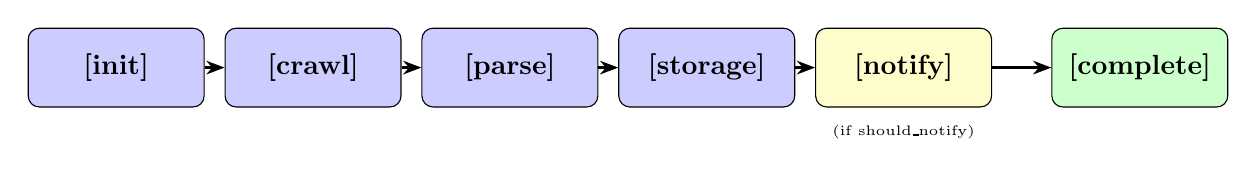
\begin{tikzpicture}[
    state/.style={rectangle, draw, fill=blue!20, text width=2cm, minimum height=1cm, align=center, rounded corners},
    arrow/.style={-Stealth, thick}
]
    % 状态节点 - 横向排列
    \node[state] (init) at (0, 0) {\textbf{[init]}};
    \node[state] (crawl) at (2.5, 0) {\textbf{[crawl]}};
    \node[state] (parse) at (5, 0) {\textbf{[parse]}};
    \node[state] (storage) at (7.5, 0) {\textbf{[storage]}};
    \node[state, fill=yellow!20] (notify) at (10, 0) {\textbf{[notify]}};
    \node[state, fill=green!20] (complete) at (13, 0) {\textbf{[complete]}};

    % 主流程箭头 - 横向
    \draw[arrow] (init) -- (crawl);
    \draw[arrow] (crawl) -- (parse);
    \draw[arrow] (parse) -- (storage);
    \draw[arrow] (storage) -- (notify);
    \draw[arrow] (notify) -- (complete);

    % 条件标注
    \node[below=0.1cm of notify, font=\tiny] {(if should\_notify)};
\end{tikzpicture}
\caption{State Transition: System state machine showing transition from initialization to completion.}
\label{fig:statetransition}
\end{figure}

\textbf{错误恢复机制}:每个节点都实现了独立的错误捕获和记录,即使某个节点失败也会继续执行后续节点。决策函数根据错误数量和状态判断是否继续,错误过多(>10个)或无数据时自动终止。

\subsection{反馈学习闭环}

系统设计了基础的反馈学习机制,形成自我优化的闭环。图~\ref{fig:learningloop}展示了学习闭环的完整流程。

\begin{figure}[htbp]
\centering
\begin{tikzpicture}[
    process/.style={rectangle, draw, fill=blue!10, text width=2.5cm, minimum height=1cm, align=center, rounded corners},
    arrow/.style={-Stealth, thick}
]
    % 主流程节点
    \node[process, fill=green!10] (task) at (0, 0) {\textbf{新任务}};

    \node[process, fill=yellow!10] (search) at (3, 0) {\textbf{模式检索}};

    \node[process, fill=orange!10] (crawl) at (6, 0) {\textbf{执行爬取}};

    \node[process, fill=red!10] (validate) at (9, 0) {\textbf{结果验证}};

    \node[process, fill=purple!10] (store) at (12, 0) {\textbf{知识存储}};

    % 反馈循环
    \node[process, fill=blue!10] (optimize) at (6, -2) {\textbf{模式优化与反馈}};

    % 主流程箭头
    \draw[arrow] (task) -- (search);
    \draw[arrow] (search) -- (crawl);
    \draw[arrow] (crawl) -- (validate);
    \draw[arrow] (validate) -- (store);

    % 反馈箭头
    \draw[arrow] (validate.south) -- (optimize.west);
    \draw[arrow] (optimize.east) to[out=0,in=270] (task.south);
\end{tikzpicture}
\caption{Learning Loop: Feedback mechanism showing continuous pattern optimization through experience accumulation.}
\label{fig:learningloop}
\end{figure}

\section{未来开发目标}

由于项目目前处于快速开发和架构重构阶段,部分设计仍在迭代中。以下是根据现有调研梳理的后续优化方向:

\begin{itemize}
    \item[$\square$] 完善模式自动优化算法,实现自适应参数调优
    \item[$\square$] 实现对爬虫特征主动学习,特攻训练蒸馏小模型
    \item[$\square$] 支持图片、音频播客、视频等内容提取,增强多模态支持
    \item[$\square$] 构建内容知识图谱,实现语义关联分析
    \item[$\square$] 实现自动A/B测试,优化爬取策略
\end{itemize}

\section{总结}

MoAgent项目初步实现了基于多智能体协作的网络信息获取系统
这是我对AI Agent的一次初步探索,旨在通过引入多智能体协作、RAG等新方法,尝试解决传统爬虫的核心痛点,赋予新时代信息获取的新方案。
目前我已搭建起基础原型并观察到一些有限进展,但整个系统仍处于早期阶段,其稳定性、泛化能力和大规模测试下的有效性还在持续验证与净化之中。
我将保持不断学习的心态,积极迭代,致力于构建更鲁棒、更实用的解决方案。

\appendix

\section{附录}

\subsection{附录A:多智能体爬虫运行实例}

图~\ref{fig:multiagent}展示了多智能体系统的完整架构,包括Supervisor和四个专业Agent的协作关系。

\begin{figure}[htbp]
\centering
\includegraphics[width=0.95\textwidth]{MulAgentresult.png}
\label{fig:multiagent}
\end{figure}

\subsection{附录B:常规爬虫工作流程}

图~\ref{fig:crawler}展示了常规爬虫的工作流程,包括HTML解析、LLM模式生成、数据提取和存储机制。

\begin{figure}[htbp]
\centering
\includegraphics[width=0.7\textwidth]{normalcrawlerresult.png}
\label{fig:crawler}
\end{figure}

\end{document}
